\documentclass[12pt]{article}

\title{CR3BP Overview}
\author{Yannis ABDELOUAHAB}
\date{2025-2026}
\usepackage[a4paper, total={7in,9in}]{geometry}
\usepackage{graphicx}
\usepackage[french]{babel}
\usepackage{amsmath}
\usepackage[]{tcolorbox}
\usepackage[]{float}
\usepackage{wrapfig}
\usepackage{interval}
\graphicspath{{../images/}}

\DeclareMathOperator{\sign}{sign}



\begin{document}
	\maketitle
	\tableofcontents
	
	\begin{abstract}
		Le problème à trois corps restreint (CR3BP en anglais) est l'étude du mouvement relatif de trois masses, dont une de masse négligeable devant les trois autres. Nous chercherons à déterminer les coordonnées des Points Lagrange, qui sont cinq points d'équilibre du CR3BP. Nous mènerons ensuite une étude de leur stabilité. A terme, nous chercherons à déterminer des orbites périodiques autour des points L1 et L2 en particulier, ainsi que mener une recherche de trajectoires de transfert qui ferait utilisation des variétés stables et instables liées aux Points Lagrange.
	\end{abstract}
	
	\section{Coordonnées des Points Lagrange}
	\subsection{Définition du système}
	\label{def_system}
	Nous étudions le système \emph{satellite de masse m} que l'on associe au point matériel $M$. On se place dans le référentiel galiléen -- que l'on note $R_G$ -- qui à pour centre le barycentre des deux masses $M_1$ et $M_2$ qu'on confondera avec le point matériel auquel leur astre respectif est associé.
	
	On cherche à exprimer les coordonnées de $M$ dans le référentiel \textit{non-galiléen} -- $R_{NG}$ -- en rotation dans le référentiel galiléen $R_G$ pour simplifier les équations du mouvement. $R_{NG}$ est alors défini comme le référentiel dans lequel $M_1$ et $M_2$ sont immobiles. On mènera la majorité de notre étude dans ce référentiel.
	
	\subsection{Expression du potentiel effectif dans $R_{NG}$}
	On cherche à déterminer les coordonnées d'un point $(x,y)$ dans $R_{NG}$. On note $(\vec{e}_x,\vec{e}_y)$ une base de $R_{G}$ et $(\vec{u}_x,\vec{u}_y)$ une base de $R_{NG}$, les deux en coordonnées cartésiennes. On note $\alpha$ l'angle entre $R_G$ et $R_{NG}$, ainsi que $\omega$ la vitesse angulaire de $R_{NG}$ par rapport à $R_G$, que l'on suppose constante. Notons $U$ l'énergie potentielle associée à $M_1$ et $M_2$. On a alors dans le référentiel galiléen $\vec{F} = -\vec{\nabla} U$ où $\vec{F}$ est la résultante des forces de gravitation, ce qui se traduit par le système :
	\begin{large}
		\begin{equation}
			\label{potential_gal}
			\begin{cases}
				m\ddot{X}=-\frac{\partial{U}}{\partial{X}} 
				\ =: \mathcal{U}_X \\
				m\ddot{Y}=-\frac{\partial{U}}{\partial{X}}
				\ =: \mathcal{U}_Y
			\end{cases}
		\end{equation}
	\end{large}
	où $(X,Y)$ sont les coordonnées d'un point $P$ dans $R_G$. On note $(x,y)$ ses coordonnées dans $R_{NG}$. On a alors $x=X\cos(\alpha)\vec{u}_x+Y\sin(\alpha)\vec{u}_y$ et $y=-X\sin(\alpha)\vec{u}_x+Y\cos(\alpha)\vec{u}_y$, ce qui se traduit matriciellement par 
	\begin{equation}
		\label{coord_change}
		\begin{pmatrix}
			x \\ y
		\end{pmatrix}
		=
		\begin{pmatrix}
			\cos(\alpha) & \sin(\alpha)
			\\
			-\sin(\alpha) & \cos(\alpha)
		\end{pmatrix}
		\begin{pmatrix}
			X \\ Y
		\end{pmatrix}
	\end{equation}
	C'est une matrice inversible dont l'inverse est 		$\begin{pmatrix}
		\cos(\alpha) & -\sin(\alpha)
		\\
		\sin(\alpha) & \cos(\alpha)
	\end{pmatrix}=:A_t$. Cette dernière vérifie donc l'équation $\begin{pmatrix}
	X\\Y
	\end{pmatrix}
	=
	A_t \begin{pmatrix}
		x\\y
	\end{pmatrix}
	$.
	
	On cherche maintenant à calculer $\begin{pmatrix}
		\ddot{X} \\ \ddot{Y}
	\end{pmatrix}$.
	On détermine d'abord $\dot{A_t}$. Comme $\alpha=\omega t$ (en prenant $\alpha(t=0)=0$), on obtient immédiatement que $\dot{A_t} = \begin{pmatrix}
		-\omega \sin(\omega t) & -\omega \cos(\omega t) \\
		\omega \cos(\omega t) & -\omega \sin(\omega t) \\
	\end{pmatrix}=-\omega J A_t$ 
	\ où \
	$J=\begin{pmatrix}
	0 & 1 \\ -1 & 0
	\end{pmatrix}$. On en déduit que :
	
	\begin{equation}
		\label{acceleration_inertial}
	\begin{pmatrix}
		\ddot{X} \\ \ddot{Y}
	\end{pmatrix}
	=
	A_t
	\begin{pmatrix}
		\ddot{x} - 2\omega\dot{y} - \omega^2x \\
		\ddot{y} + 2\omega\dot{x} - \omega^2y
	\end{pmatrix}
	\end{equation}
	
	Avec l'équation \ref{potential_gal} multipliée par $A_t^{-1}$ on a 
	$m A_t^{-1}
	\begin{pmatrix}
		\ddot{X} \\ \ddot{Y}
	\end{pmatrix} 
	=
	-A_t^{-1} \begin{pmatrix}
		\mathcal{U}_X \\ \mathcal{U}_Y
	\end{pmatrix}
	$. Le membre de gauche se simplifie en $m \times$ le membre de gauche de l'équation \ref{acceleration_inertial}. Le membre de droite correspond cependant au changement de base de la dérivée de l'énergie potentielle : le membre de droite devient $-\begin{pmatrix}
		\mathcal{U}_x
		\\ \mathcal{U}_y
	\end{pmatrix}$. En posant $\bar{\mathcal{U}}_x := -\mathcal{U}_x + m\omega^2x$ et $\bar{\mathcal{U}}_y := -\mathcal{U}_y + m\omega^2y$,
	on obtient finalement les équations du mouvement suivantes :
	\begin{equation}
		\begin{cases}
			\ddot{x} - 2\omega\dot{y} = - \frac{1}{m}\bar{\mathcal{U}}_x \\
			\ddot{y} + 2\omega\dot{x} = - \frac{1}{m}\bar{\mathcal{U}}_y
		\end{cases}
	\end{equation}
	ainsi que l'équation de l'énergie potentielle effective dans $R_{NG}$ :

	\begin{tcolorbox}[colframe=black,boxrule=0.8pt,colback=white]
	\begin{equation}
		\bar{U} = U(x,y) - \frac{1}{2}m\omega^2(x^2+y^2)
	\end{equation}
	\end{tcolorbox}
	
	On peut tracer ce potentiel à l'aide du programme python en annexe (INSERT ANNEXE HERE). On obtient alors la figure suivante :
	\begin{figure}[H]
		\centering
		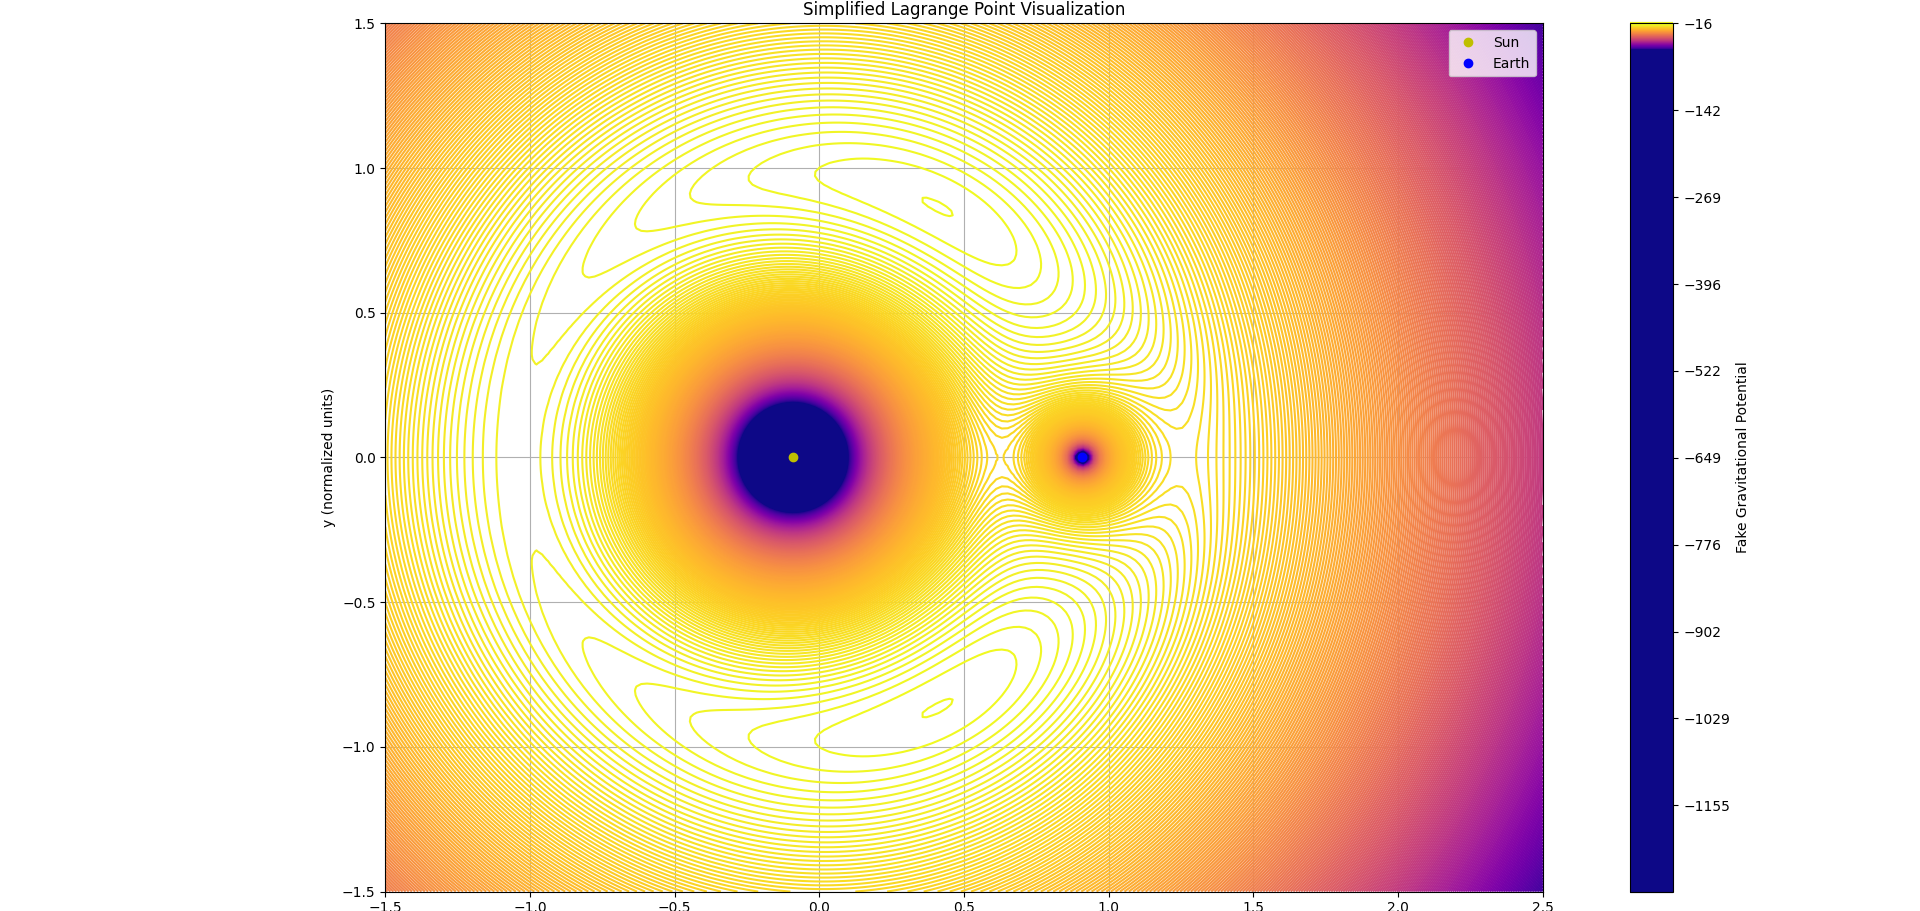
\includegraphics[width=0.75\linewidth]{potential_clear.png}
		\caption{A nice potential.}
		\label{fig:orbits1}
	\end{figure}
	
	
	\subsection{Coordonnées des points colinéaires}
	On cherche dans cette section à déterminer les coordonnées des points colinéaires, i.e. ceux que l'on peut observer sur l'axe des abscisses dans la figure (\ref{fig:orbits1}). Ainsi, dans cette partie, nous travaillerons en supposant aucun mouvement vertical : $\forall t$, $y(t)=0$, $v_y(t)=0$ and $a_y(t)=0$. Les points d'équilibres colinéaires correspondent ici aux points d'annulations de la dérivé de $\bar{U}(x,0)$ par rapport à $x$. Notons $\mu := \frac{M_2}{M_1+M_2}$ le coefficient de masse du sysème. Ainsi, le barycentre du système étant placé en $(0,0)$, on a :
	\begin{equation}
		\label{potential_in_y=0}
		\bar{U}(x,0)=-\frac{1}{2}m\omega^2x^2-\frac{GmM_1}{|x+\mu R|}-\frac{GmM_2}{|x-(1-\mu)R|}
	\end{equation}
	et en dérivant :
	\begin{equation}
		\label{bilan_force_y=0}
		\frac{\partial \bar{U}}{\partial x}=-m\omega^2x+\frac{GmM_1}{(x+\mu R)^2}\sign(x+\mu R)+\frac{GmM_2}{(x-(1-\mu)R)^2}\sign(x-(1-\mu)R)
	\end{equation}
	\begin{figure}[H]
		\centering
		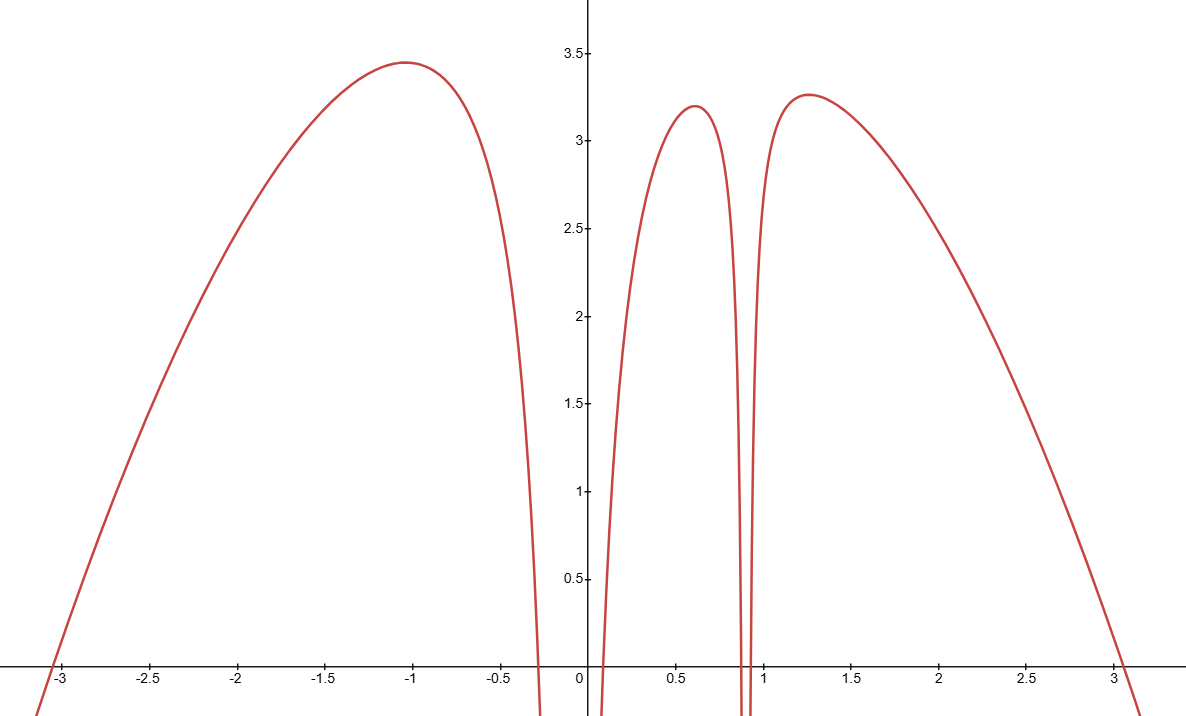
\includegraphics[width=0.4\textwidth]{colinear-graph.png}
		\caption{Le potentiel effectif selon $x$ en $y=0$.}
		\label{fig:potential_in_x}
	\end{figure}
	En traçant ce potentiel, on obtient alors la figure \ref{fig:potential_in_x} précédente, sur laquelle on peut en observer la présence des trois points d'équilibre que l'on recherche. On les nommera $L3$, $L1$ et $L2$ selon leur ordre d'apparition sur la figure \ref{fig:potential_in_x}. On cherche maintenant à déterminer les points d'annulation du potentiel effectif (i.e. les points d'équilibres précédemment mentionnés). Pour ce faire, nous travaillerons avec l'hypothèse que $\mu \to 0^+$ qui nous simplifiera la résolution des calculs. Il peut être montré (pas discuté ici) que le polynôme de degré cinq, qui apparait lors de la résolution analytique des points d'annulation de la formule \ref{bilan_force_y=0}, n'admet pas de racine calculable (cf. The Lagrange Points by Neil J. Cornish). On distingue trois cas.
	
	
	\subsubsection{Coordonnées de L1}
	On cherche ici à déterminer les coordonnées du point L1. Ce point ce situe entre $M_1$ et $M_2$. On prend alors $x \in \interval[open]{-\mu}{1-\mu}$. Sur cet intervalle, on a $x+\mu R>0$ et $x-(1-\mu)R<0$. En utilisant la forme dérivé de l'équation \ref{potential_in_y=0} et en se plaçant sur le segment considéré, la condition nécessaire d'équilibre s'écrit :
	\begin{equation}
		\label{L1_equilibrium_eq}
		\omega^2x - \frac{GM_1}{(x+\mu R)^2} + \frac{GM_2}{(x-(1-\mu)R)^2} = 0
	\end{equation}
	On peut noter que les masses se simplifient.
	Du fait que l'on suppose $\mu \to 0$, on peut affirmer qualitativement que le point d'équilibre est bien plus proche de $M_2$ que de $M_1$, sous peine que l'attraction de $M_2$ soit négligeable devant celle de $M_1$. On pose alors $\varepsilon := x - (1-\mu)R$ la distance entre $M_2$ et L1. Ici, on s'attend à ce que $\varepsilon < 0$ dû à l'orientation du référentiel. On obtient ainsi :
	\begin{equation}
		\omega^2((1-\mu)R+\varepsilon) - \frac{GM_1}{(R+\varepsilon)^2} + \frac{GM_2}{\varepsilon^2} = 0
	\end{equation}
	On peut alors procéder à un DL à l'ordre 1 en $\varepsilon$ (car on a émis l'hypothèse $\varepsilon \to 1$) ce qui, après quelques calculs longs donne :
	\begin{equation}
		\frac{\varepsilon}{R^3}(3M_1+M_2)+\frac{M_2}{\varepsilon^2}=0 \implies \varepsilon = -(\frac{M_2}{3M_1+M_2})^\frac{1}{3}R
	\end{equation}
	
	
	\subsubsection{Coordonnées de L2}
	Déterminer les coordonnées de L2 est très similaire au processus pour L1. Dans ce cas, le point se trouve à l'opposé de $M_2$ par rapport à $M_1$. Ainsi on a $x \in \interval[open]{1-\mu}{+\infty}$. Sur cet intervalle, on a $x+\mu R>0$ et $x-(1-\mu)R>0$. On peut ainsi écrire comme précédemment l'équation liée à la condition nécessaire d'équilibre. Pour L2, nous pouvons reposer le même $\varepsilon$ et tenir le même raisonnement pour obtenir au final que
	\begin{equation}
		\varepsilon = +(\frac{M_2}{3M_1+M_2})^\frac{1}{3}R
	\end{equation}
	Dans ce cas, on peut raisonner à nouveau qualitativement pour justifier ce $\varepsilon$. Le point L2 se situe au delà de l'astre $M_2$ ce qui implique que l'attraction de $M_2$ et celle de $M_1$ attire dans le sens $M \to M_2$ (où M est le point matériel associé au satellite, défini ainsi au \ref{def_system}). Or, si l'on se place loin de $M_2$, seul l'attraction de $M_1$ sera ressentie, ce qui revient à traiter le problème à 2-corps, et on peut facilement montrer que l'on obtient une orbite pour laquelle la coordonnée en y dans $R_{NG}$ est non constante égale à 0. Donc on n'aurait pas à faire à un point d'équilibre. Il faut ainsi se placer proche de $M_2$.
	
	
	\subsubsection{Coordonnées de L3}
	Dernier des points colinéaires, L3 est bien différent de ses deux frères L1 et L2. Ce point se positionne de l'autre côté de $M_1$ par rapport à $M_2$, et se situe, comme l'on va le voir, environ à la même distance de $M_1$ que $M_2$.
	On a alors $x \in \interval[open]{-\infty}{-\mu}$. Sur cet intervalle, on se retrouve avec $x+\mu R<0$ et $x-(1-\mu)R<0$, ce qui se traduit dans l'équation liée à la condition nécessaire d'équilibre par :
	\begin{equation}
		\label{L3_equilibrium_eq}
		\omega^2x + \frac{GM_1}{(x+\mu R)^2} + \frac{GM_2}{(x-(1-\mu)R)^2} = 0
	\end{equation}
	Or, avec l'hypothèse que $\mu \to 0$, qui se traduit par $M_2 << M_1$, on obtient l'approximation $x + \frac{GM_1}{(x+\mu R)^2}=0$ d'où $x \approx -R$. On cherche maintenant à déterminer l'écart que l'on note $\delta$ entre l'approximation et la véritable position d'équilibre. On a alors $x = \delta-R$. En remplaçant dans \ref{L3_equilibrium_eq} on a :
	\begin{equation}
		\omega^2(\delta-R) + \frac{GM_1}{(\delta-(1-\mu)R)^2}+\frac{GM_2}{(\delta-(2-\mu)R)^2} = 0
	\end{equation}
	On peut maintenant procéder à résoudre pour $\delta$ à l'aide de deux développements limités, un sur chacun des deux termes droits (DL en $\frac{\delta}{R}+\mu$). On peut ainsi montrer que :
	\begin{equation}
		\delta = \frac{(\frac{3}{4}-\frac{\mu}{4})M_2-2\mu M_1}{3M_1+\frac{5}{4}M_2}
	\end{equation}

	
	
	
\end{document}